%!TEX root = ../dokumentation.tex
\section{Projekorganisation}

\begin{figure}[!ht]
\begin{center}
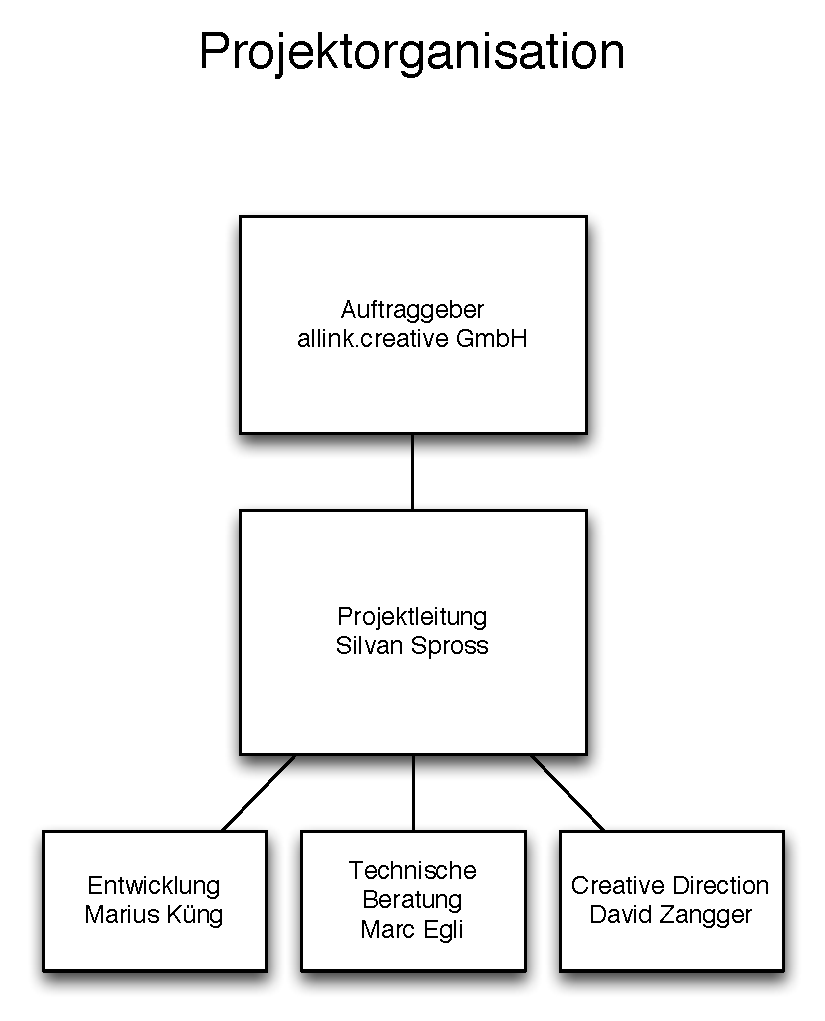
\includegraphics[width=0.5\textwidth,angle=0]{./bilder/01_projektorganisation.pdf}
\caption[Projekorganisation]{Projekorganisation\footnotemark}
\end{center}
\end{figure}
\footnotetext{Eigene Darstellung}

\section{Vorkenntnisse}

Technologien
\begin{itemize}
    \item Python Grundkenntnisse
    \item Django fortgeschrittene Kenntnisse
    \item Piston Grundkenntnisse
    \item jQuery fortgeschrittene Kenntnisse
    \item HTML5 gute Kenntnisse
    \item CSS3 gute Kenntnisse
    \item AJAX fortgeschrittene Kenntnisse\\
\end{itemize}

Anwendungen
\begin{itemize}
    \item Mehrere komplette Webauftritte realisiert
    \item Applikationen in Django erstellt (News, Blog, Produkteübersicht)
    \item Schnittstellen programmiert (XML, JSON)
    \item Per AJAX dynamische Inhalte laden und einfügen
    \item Dynamische Formulare abschicken und Request entgegennehmen
    \item DOM-Elemente manipulieren, per Events steuern
\end{itemize}
    
\section{Vorarbeiten}
Ich habe, um einen ersten Eindruck über die Funktionalität zu erhalten, den bestehenden yatplaner ausprobiert.
Ansonsten fand keine explizite Vorarbeit statt.

\section{Firmenstandards}
\begin{itemize}
    \item Betriebsystem: Mac OS X
    \item Editor: Textmate
    \item Entwicklungsumgebung: Python, Django (Python-Framework für Webapplikationen)
    \item Lokale Testumgebung: Django Server
    \item Deployment: per fabric-script auf Apache-Server
    \item Versionierung: Git, auf Github veröffentlicht
\end{itemize}
\clearpage
\section{Zeitplan}
Ich plante in einzelnen Schritten oder fasste gewisse Aufgaben zusammen und schätzte wie lange ich an einem Feature brauchen würde.
Dazwischen habe ich mir Meilensteine gesetzt mit einem Datum, dass ich einzuhalten plante.
In der Planung habe ich bei kleinen Aufgaben meist zu viel geplant und dann in der Realität diese Überzeit aufgestockt. Damit wurde mehr Zeit für die Realisierung frei.\\
\begin{table}[!ht]
\begin{center}
    \begin{tabular}{lll}
        \toprule Beschreibung & Planung & Realität \\
        \midrule Teil 1 & &\\
        \midrule Zeitplan erstellen & 2 & 2\\
        \midrule Dokumentation gliedern & 1 & 1\\
        \midrule Aufgabenstellung erfassen & 1 & 0.25\\
        \midrule Projektorganisation erfassen  & 1 & 0.25\\
        \midrule Vorkenntnisse erfassen & 1 & 1\\
        \midrule Vorarbeiten erfassen & 1 & 0.25 \\
        \midrule Deklaration des Firmenstandards erfassen & 1 & 0.5\\
        \midrule MS: Teil 1 abschliessen & 13.03. & 13.03.
     \end{tabular}
\end{center}
\end{table}
\clearpage
\begin{table}[!ht]
\begin{center}      
     \begin{tabular}{lll}\\
        \toprule Beschreibung & Planung & Realität \\
        \midrule Teil 2 & & \\
        \midrule Projektbeschreibung erfassen  & 1 & 1\\
        \midrule Systembeschreibung (Django, planer) & 1 & 0.5\\
        \midrule Analyse IST-Zustand & 1 & 1.5\\
        \midrule Definition Muss-/Kann-Ziele & 2 & 2\\
        \midrule MS: Ziele definiert & 14.03. & 14.03. \\
        \midrule MS: Planung abgeschlossen & 14.03. & 14.03. \\
        \midrule ERM erstellen & 2 & 1\\
        \midrule rails yatplaner studieren & 1 & 2\\
        \midrule Projekt aufsetzen & 1 & 0.5\\
        \midrule Modellierung Django & 1.5 & 1\\
        \midrule MS: Modellierung & 14.03. & 14.03.\\
        \midrule View erstellen & 4 & 3\\
        \midrule Tabelle Template (nur HTML) (Wochenansicht) & 3 & 2\\
        \midrule Daten in Tabelle einsetzen & 3 & 2\\
        \midrule Wochenansicht ausarbeiten & 7 & 7\\
        \midrule JS Funktionalität einbinden (Ajax) (MUSS) & 8 & 8\\
        \midrule MS: POST per AJAX schicken & 16.03. & 16.03.\\
        \midrule Bugfixing & 5 & 6\\
        \midrule Realisierung beschreiben & 3 & 6\\
        \midrule MS: MUSS-Ziele erreicht & 21.03. & 20.03.\\
        \midrule MS: Prototyp & 21.03. & 20.03.\\
     \end{tabular}
\end{center}
\end{table}
\clearpage
\begin{table}[!ht]
\begin{center}      
     \begin{tabular}{lll}
        \toprule Beschreibung & Planung & Realität \\
        \midrule Kann-Ziele & 16 & 16\\
        \midrule MS: KANN-Ziele erreicht & 26.03. & 23.03.\\
        \midrule Testfälle erstellen & 1 & 1\\
        \midrule Testing im allink.planer & 1 & 0.5\\
        \midrule Testfälle dokumentieren & 1 & 0.5\\
        \midrule Bugfixing & 3 & 2\\
        \midrule Codesäuberungen & 0.5 & 0.5\\
        \midrule Implementierung in allink.planer (master) & 0.5 & 0.25\\
        \midrule MS: Realisierung & 26.03. & 23.03.\\
        \midrule Erreichte Ziele erfassen (Muss-Ziele, Kann-Ziele) & 1 & 1\\
        \midrule Websummary online erfassen & 1 & 1.5\\
        \midrule Quellenangabe & 1 & 1\\
        \midrule Glossar & 0.5 & 2\\
        \midrule Dokumentation abschliessen & 1 & 4\\
        \midrule Arbeit einreichen & 2 & 1\\
        \midrule & &\\
        \midrule Total & 80 & 80\\
        \bottomrule
    \end{tabular}
    \caption{Zeitplan}
\end{center}
\end{table}
